\documentclass[11pt,spanish]{beamer}
\usepackage{mathpazo}
\usepackage{tgheros}
\renewcommand{\familydefault}{\sfdefault}
\usepackage[T1]{fontenc}
\usepackage[utf8]{inputenc}
\usepackage{babel}
\usepackage{amsmath}
\usepackage{amssymb}
\usepackage{array}
\usepackage{tikz}
\usetikzlibrary{arrows.meta,calc,positioning,shapes.geometric}

\definecolor{Guinda}{rgb}{0.49, 0.05, 0.12}
\definecolor{Rojo}{rgb}{0.8, 0, 0}
\definecolor{indiagreen}{rgb}{0.07,0.53,0.03}
\definecolor{anti-flashwhite}{rgb}{0.95,0.95,0.96}
\definecolor{pastelblue}{rgb}{0.78,0.87,0.96}
\definecolor{pastelgreen}{rgb}{0.82,0.92,0.78}
\definecolor{pastelpeach}{rgb}{0.98,0.84,0.72}
\definecolor{pastelrose}{rgb}{0.96,0.78,0.84}
\definecolor{pastelviolet}{rgb}{0.86,0.80,0.96}
\definecolor{pastelyellow}{rgb}{0.98,0.93,0.70}

\usecolortheme[named=indiagreen]{structure}
\usetheme{Boadilla}
\usefonttheme{structurebold}
\setbeamertemplate{itemize items}[default]
\setbeamertemplate{enumerate items}[default]
\setbeamertemplate{navigation symbols}{}
\setbeamercolor{block title}{fg=white,bg=indiagreen!85!black}
\setbeamercolor{block body}{fg=black,bg=pastelgreen!45!white}

\hypersetup{hidelinks}
\addto\shorthandsspanish{\spanishdeactivate{~<>.}}
\newcommand{\term}[1]{\textbf{\textcolor{indiagreen!80!black}{#1}}}
\newcommand{\actividad}[1]{\textbf{\textcolor{Rojo}{#1}}}
\newcolumntype{L}[1]{>{\raggedright\arraybackslash}p{#1}}

\hyphenpenalty=9000
\exhyphenpenalty=9000
\emergencystretch=2em

\tikzset{
  idea/.style={
    rounded corners=3pt,
    draw=indiagreen!70!black,
    fill=pastelgreen,
    align=center,
    inner sep=7pt,
    font=\small
  },
  bloque/.style={
    rounded corners=3pt,
    draw=black!35,
    fill=pastelblue,
    align=center,
    text width=2.8cm,
    minimum height=1.05cm,
    inner sep=5pt,
    font=\small
  },
  mini/.style={
    rounded corners=3pt,
    draw=black!35,
    fill=anti-flashwhite,
    align=center,
    text width=2.35cm,
    minimum height=.85cm,
    inner sep=4pt,
    font=\scriptsize
  },
  paso/.style={
    rounded corners=3pt,
    draw=indiagreen!70!black,
    fill=pastelgreen,
    align=center,
    text width=2.05cm,
    minimum height=.95cm,
    inner sep=4pt,
    font=\scriptsize
  },
  arrow/.style={
    -{Stealth[length=2.5mm]},
    thick,
    indiagreen!80!black
  }
}

\title[PDS]{\textbf{Del software de sistemas al análisis léxico}}
\subtitle{Repaso de las notas 02 y 03 y trabajo con el Cuadernillo 02%
\ifkahoot\else\\[0.35em]\textit{Versión sin kahoot}\fi}
\author[Soto Romero y Reyes Cabello]{Manuel Soto Romero \and Araceli Liliana Reyes Cabello}
\institute[UACM]{Colegio de Ciencia y Tecnología, UACM}
\date{Semestre 2026-2}

\begin{document}

\begin{frame}
\titlepage
\end{frame}

\ifkahoot
\begin{frame}{Iniciamos con \textsc{Kahoot}}
\vfill

\begin{center}
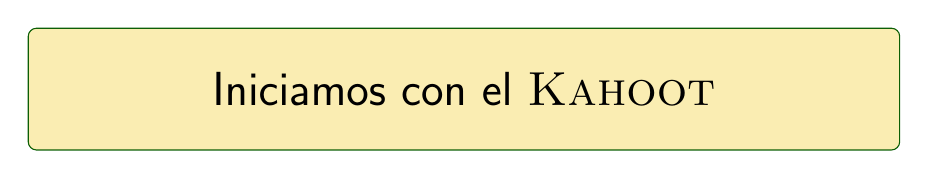
\begin{tikzpicture}
\node[
  idea,
  fill=pastelyellow,
  text width=.82\textwidth,
  inner sep=16pt,
  font=\LARGE
]
{Iniciamos con el \textsc{Kahoot}};
\end{tikzpicture}
\end{center}

\vfill
\end{frame}
\fi

\begin{frame}{Ruta de trabajo}
\vfill

\begin{center}
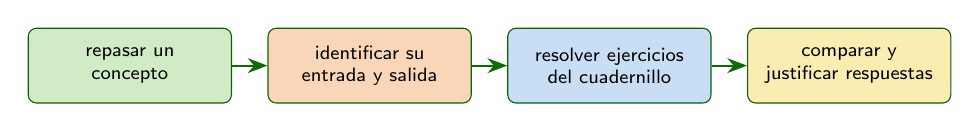
\begin{tikzpicture}[node distance=.45cm]
\node[paso, fill=pastelgreen, text width=2.3cm] (a) {repasar un\\concepto};
\node[paso, fill=pastelpeach, right=of a, text width=2.3cm] (b) {identificar su\\entrada y salida};
\node[paso, fill=pastelblue, right=of b, text width=2.3cm] (c) {resolver ejercicios\\del cuadernillo};
\node[paso, fill=pastelyellow, right=of c, text width=2.3cm] (d) {comparar y\\justificar respuestas};
\draw[arrow] (a) -- (b);
\draw[arrow] (b) -- (c);
\draw[arrow] (c) -- (d);
\end{tikzpicture}
\end{center}

\bigskip

\begin{block}{Durante la sesión}
Alternaremos el repaso de las notas 02 y 03 con el trabajo del \term{Cuadernillo de ejercicios 02}.
\end{block}

\vfill
\end{frame}

\begin{frame}{Abrimos la caja del compilador}
\vfill

\begin{center}
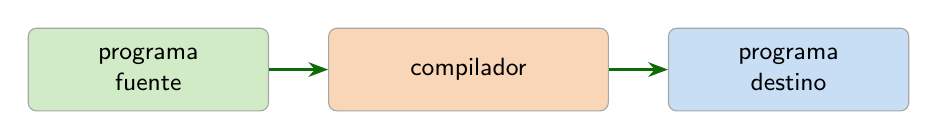
\begin{tikzpicture}[node distance=.75cm]
\node[bloque, fill=pastelgreen, text width=2.7cm] (a) {programa\\fuente};
\node[bloque, fill=pastelpeach, right=of a, text width=3.2cm] (b) {compilador};
\node[bloque, fill=pastelblue, right=of b, text width=2.7cm] (c) {programa\\destino};
\draw[arrow] (a) -- (b);
\draw[arrow] (b) -- (c);
\end{tikzpicture}
\end{center}

\bigskip

\begin{block}{La descripción externa no basta}
En su interior, el compilador reconoce unidades, descubre estructuras, comprueba restricciones y transforma representaciones antes de producir su salida.
\end{block}

\bigskip

\begin{center}
\term{El programa cambia de representación, pero debe conservar su significado.}
\end{center}

\vfill
\end{frame}

\begin{frame}{Dos grandes etapas: análisis y síntesis}
\vfill

\begin{columns}[T,onlytextwidth]
\begin{column}{.48\textwidth}
\begin{block}{Análisis}
\small
Examina el programa fuente para reconocer sus componentes, su estructura y las restricciones que debe satisfacer.
\end{block}
\end{column}
\begin{column}{.48\textwidth}
\begin{block}{Síntesis}
\small
Toma la representación obtenida por el análisis y construye una representación equivalente en el lenguaje destino.
\end{block}
\end{column}
\end{columns}

\bigskip

\begin{center}
\resizebox{.96\textwidth}{!}{%
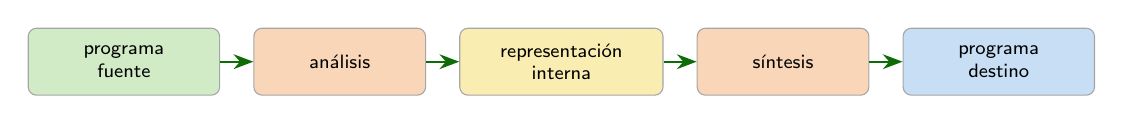
\begin{tikzpicture}[node distance=.42cm]
\node[mini, fill=pastelgreen, text width=2.15cm] (a) {programa\\fuente};
\node[mini, fill=pastelpeach, right=of a, text width=1.9cm] (b) {análisis};
\node[mini, fill=pastelyellow, right=of b, text width=2.3cm] (c) {representación\\interna};
\node[mini, fill=pastelpeach, right=of c, text width=1.9cm] (d) {síntesis};
\node[mini, fill=pastelblue, right=of d, text width=2.15cm] (e) {programa\\destino};
\draw[arrow] (a) -- (b);
\draw[arrow] (b) -- (c);
\draw[arrow] (c) -- (d);
\draw[arrow] (d) -- (e);
\end{tikzpicture}%
}
\end{center}

\vfill
\end{frame}

\begin{frame}{Las fases se comunican mediante contratos}
\vfill

\begin{center}
\scriptsize
\renewcommand{\arraystretch}{1.18}
\begin{tabular}{|L{.22\textwidth}|L{.28\textwidth}|L{.37\textwidth}|}
\hline
\textbf{Fase} & \textbf{Entrada} & \textbf{Salida principal} \tabularnewline
\hline
Análisis léxico & Caracteres & Secuencia de tokens \tabularnewline
\hline
Análisis sintáctico & Tokens & Representación estructurada \tabularnewline
\hline
Análisis semántico & Estructura e información necesaria & Representación comprobada \tabularnewline
\hline
Generación de IR & Representación comprobada & Representación intermedia \tabularnewline
\hline
Optimización & Representación intermedia & Representación equivalente \tabularnewline
\hline
Generación de código & Representación validada o intermedia & Programa destino \tabularnewline
\hline
\end{tabular}
\end{center}

\bigskip

\begin{block}{Pregunta para cada fase}
¿Qué recibe?, ¿qué tarea realiza?, ¿qué produce? y ¿quién utiliza el resultado?
\end{block}

\vfill
\end{frame}

\begin{frame}{Trabajo con el cuadernillo}
\vfill

\begin{center}
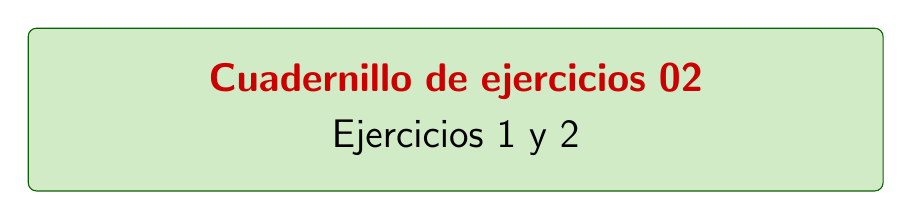
\begin{tikzpicture}
\node[
  idea,
  fill=pastelgreen,
  text width=.82\textwidth,
  inner sep=13pt,
  font=\Large
]
{\actividad{Cuadernillo de ejercicios 02}\\[2pt]
Ejercicios 1 y 2};
\end{tikzpicture}
\end{center}

\bigskip

\begin{itemize}
\item \textbf{Esencial --- Ejercicio 1:} reconocer los contratos entre fases.
\item \textbf{Extensión --- Ejercicio 2:} distinguir las tareas de análisis y de síntesis.
\end{itemize}

\vfill
\end{frame}

\begin{frame}{Tres fases para comprender el programa fuente}
\vfill

\begin{center}
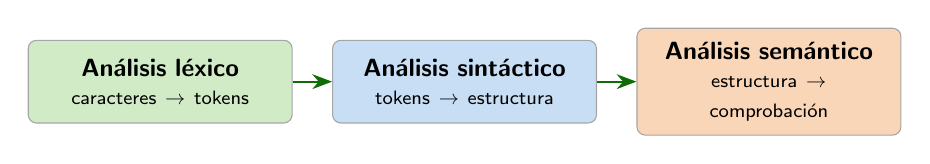
\begin{tikzpicture}[node distance=.5cm]
\node[bloque, fill=pastelgreen, text width=3cm] (a) {\textbf{Análisis léxico}\\[-1pt]\scriptsize caracteres \(\rightarrow\) tokens};
\node[bloque, fill=pastelblue, right=of a, text width=3cm] (b) {\textbf{Análisis sintáctico}\\[-1pt]\scriptsize tokens \(\rightarrow\) estructura};
\node[bloque, fill=pastelpeach, right=of b, text width=3cm] (c) {\textbf{Análisis semántico}\\[-1pt]\scriptsize estructura \(\rightarrow\) comprobación};
\draw[arrow] (a) -- (b);
\draw[arrow] (b) -- (c);
\end{tikzpicture}
\end{center}

\bigskip

\begin{itemize}
\item El léxico reconoce unidades elementales.
\item El sintáctico organiza esas unidades según la gramática.
\item El semántico comprueba restricciones como declaraciones y compatibilidad de tipos.
\end{itemize}

\vfill
\end{frame}

\begin{frame}{Cada fase detecta problemas diferentes}
\vfill

\begin{center}
\small
\renewcommand{\arraystretch}{1.25}
\begin{tabular}{|L{.22\textwidth}|L{.65\textwidth}|}
\hline
\textbf{Fase} & \textbf{Situación que le corresponde} \tabularnewline
\hline
Léxica & Ningún patrón permite reconocer el inicio de los caracteres restantes. \tabularnewline
\hline
Sintáctica & Los tokens existen, pero no pueden organizarse de acuerdo con la gramática. \tabularnewline
\hline
Semántica & La estructura es válida, pero incumple una regla de declaración o de tipos. \tabularnewline
\hline
\end{tabular}
\end{center}

\bigskip

\begin{block}{Límite de responsabilidad}
Reconocer un texto como identificador no permite decidir todavía si fue declarado ni qué tipo tiene.
\end{block}

\vfill
\end{frame}

\begin{frame}{Trabajo con el cuadernillo}
\vfill

\begin{center}
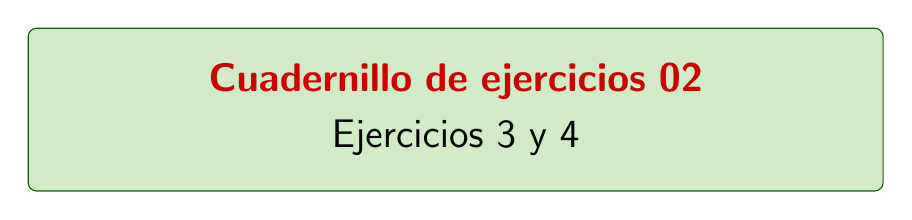
\begin{tikzpicture}
\node[
  idea,
  fill=pastelgreen,
  text width=.82\textwidth,
  inner sep=13pt,
  font=\Large
]
{\actividad{Cuadernillo de ejercicios 02}\\[2pt]
Ejercicios 3 y 4};
\end{tikzpicture}
\end{center}

\bigskip

\begin{itemize}
\item \textbf{Esencial --- Ejercicio 3:} decidir qué fase debe responder en cada situación.
\item \textbf{Extensión --- Ejercicio 4:} revisar los límites de responsabilidad entre fases.
\end{itemize}

\vfill
\end{frame}

\begin{frame}{De la representación validada al código destino}
\vfill

\begin{center}
\resizebox{.96\textwidth}{!}{%
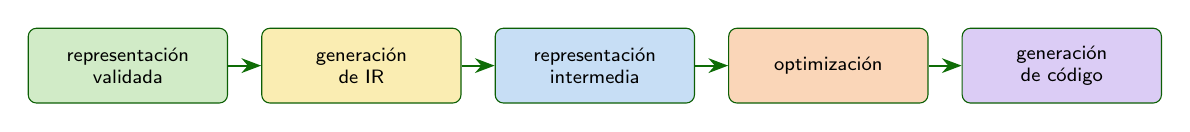
\begin{tikzpicture}[node distance=.42cm]
\node[paso, fill=pastelgreen, text width=2.25cm] (a) {representación\\validada};
\node[paso, fill=pastelyellow, right=of a, text width=2.25cm] (b) {generación\\de IR};
\node[paso, fill=pastelblue, right=of b, text width=2.25cm] (c) {representación\\intermedia};
\node[paso, fill=pastelpeach, right=of c, text width=2.25cm] (d) {optimización};
\node[paso, fill=pastelviolet, right=of d, text width=2.25cm] (e) {generación\\de código};
\draw[arrow] (a) -- (b);
\draw[arrow] (b) -- (c);
\draw[arrow] (c) -- (d);
\draw[arrow] (d) -- (e);
\end{tikzpicture}%
}
\end{center}

\bigskip

\begin{itemize}
\item Una IR facilita la comunicación y la transformación del programa.
\item La optimización busca una mejora sin cambiar el comportamiento definido.
\item No todos los compiladores usan exactamente una IR o el mismo número de optimizaciones.
\end{itemize}

\vfill
\end{frame}

\begin{frame}{El compilador del curso y la cadena posterior}
\vfill

\begin{center}
\resizebox{.96\textwidth}{!}{%
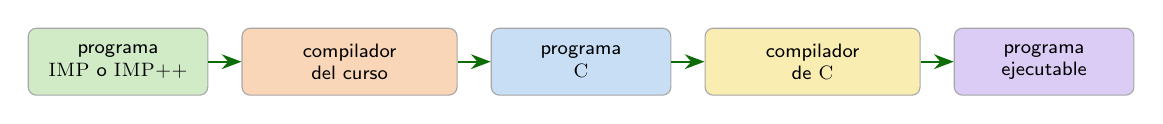
\begin{tikzpicture}[node distance=.42cm]
\node[mini, fill=pastelgreen, text width=2cm] (a) {programa\\\textsc{IMP} o \textsc{IMP++}};
\node[mini, fill=pastelpeach, right=of a, text width=2.45cm] (b) {compilador\\del curso};
\node[mini, fill=pastelblue, right=of b, text width=2cm] (c) {programa\\\textsc{C}};
\node[mini, fill=pastelyellow, right=of c, text width=2.45cm] (d) {compilador\\de \textsc{C}};
\node[mini, fill=pastelviolet, right=of d, text width=2cm] (e) {programa\\ejecutable};
\draw[arrow] (a) -- (b);
\draw[arrow] (b) -- (c);
\draw[arrow] (c) -- (d);
\draw[arrow] (d) -- (e);
\end{tikzpicture}%
}
\end{center}

\bigskip

\begin{block}{Destino de nuestro compilador}
El programa \textsc{C} completa la traducción prevista para el curso. Todavía necesita un compilador de \textsc{C} para continuar la cadena hacia un ejecutable.
\end{block}

\begin{center}
\small En clase construiremos la base \textsc{IMP}; en las prácticas la extenderemos para \textsc{IMP++}.
\end{center}

\vfill
\end{frame}

\begin{frame}{Integrar significa acordar interfaces}
\vfill

\begin{center}
\resizebox{.96\textwidth}{!}{%
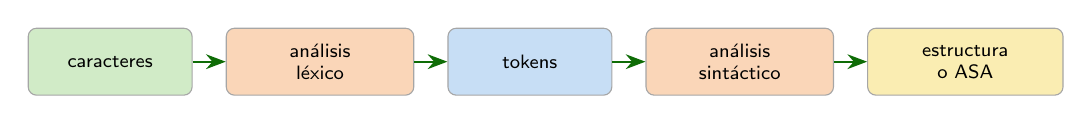
\begin{tikzpicture}[node distance=.42cm]
\node[mini, fill=pastelgreen, text width=1.8cm] (a) {caracteres};
\node[mini, fill=pastelpeach, right=of a, text width=2.1cm] (b) {análisis\\léxico};
\node[mini, fill=pastelblue, right=of b, text width=1.8cm] (c) {tokens};
\node[mini, fill=pastelpeach, right=of c, text width=2.1cm] (d) {análisis\\sintáctico};
\node[mini, fill=pastelyellow, right=of d, text width=2.2cm] (e) {estructura\\o ASA};
\draw[arrow] (a) -- (b);
\draw[arrow] (b) -- (c);
\draw[arrow] (c) -- (d);
\draw[arrow] (d) -- (e);
\end{tikzpicture}%
}
\end{center}

\bigskip

\begin{columns}[T,onlytextwidth]
\begin{column}{.48\textwidth}
\begin{block}{Contrato}
\small
La fase consumidora debe conocer la forma y el significado de los datos que recibe.
\end{block}
\end{column}
\begin{column}{.48\textwidth}
\begin{block}{Cambio}
\small
Si cambia una representación, deben revisarse las fases que la producen y la consumen.
\end{block}
\end{column}
\end{columns}

\bigskip

\begin{center}
\scriptsize ASA significa \textit{árbol de sintaxis abstracta}; la denominación proviene del inglés \textit{Abstract Syntax Tree}, abreviado AST.
\end{center}

\vfill
\end{frame}

\begin{frame}{Trabajo con el cuadernillo}
\vfill

\begin{center}
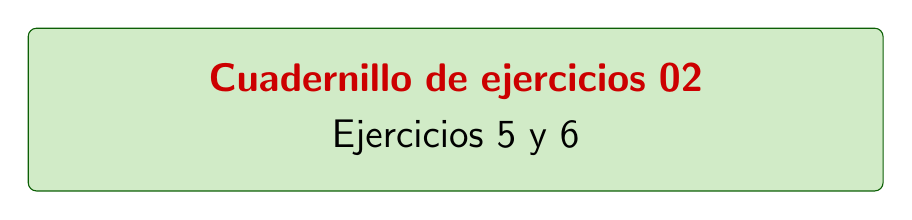
\begin{tikzpicture}
\node[
  idea,
  fill=pastelgreen,
  text width=.82\textwidth,
  inner sep=13pt,
  font=\Large
]
{\actividad{Cuadernillo de ejercicios 02}\\[2pt]
Ejercicios 5 y 6};
\end{tikzpicture}
\end{center}

\bigskip

\begin{itemize}
\item \textbf{Esencial --- Ejercicio 5:} completar el recorrido común de \textsc{IMP}/\textsc{IMP++} a \textsc{C}.
\item \textbf{Extensión --- Ejercicio 6:} analizar las interfaces y el efecto de sus cambios.
\end{itemize}

\vfill
\end{frame}

\begin{frame}{Función del analizador léxico}
\vfill

\begin{center}
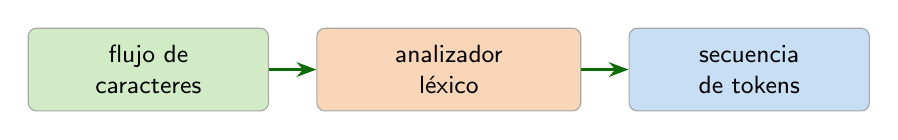
\begin{tikzpicture}[node distance=.6cm]
\node[bloque, fill=pastelgreen, text width=2.7cm] (a) {flujo de\\caracteres};
\node[bloque, fill=pastelpeach, right=of a, text width=3cm] (b) {analizador\\léxico};
\node[bloque, fill=pastelblue, right=of b, text width=2.7cm] (c) {secuencia\\de tokens};
\draw[arrow] (a) -- (b);
\draw[arrow] (b) -- (c);
\end{tikzpicture}
\end{center}

\bigskip

\begin{itemize}
\item Agrupa caracteres en lexemas y produce tokens.
\item Puede omitir espacios o comentarios cuando el lenguaje indica que no son significativos.
\item Conserva atributos necesarios para las fases posteriores.
\item No determina por sí solo la estructura completa, las declaraciones o los tipos.
\end{itemize}

\vfill
\end{frame}

\begin{frame}{Del flujo de caracteres a los tokens}
\vfill

\begin{block}{Fragmento ilustrativo: no define la sintaxis de \textsc{IMP}}
\centering
\texttt{valor = valor + inc;}
\end{block}

\bigskip

\begin{center}
\small
\renewcommand{\arraystretch}{1.18}
\begin{tabular}{|L{.22\textwidth}|L{.27\textwidth}|L{.35\textwidth}|}
\hline
\textbf{Lexema} & \textbf{Clasificación} & \textbf{Resultado descriptivo} \tabularnewline
\hline
\texttt{valor} & identificador & \texttt{ID(valor)} \tabularnewline
\hline
\texttt{=} & asignación & \texttt{ASIG} \tabularnewline
\hline
\texttt{valor} & identificador & \texttt{ID(valor)} \tabularnewline
\hline
\texttt{+} & suma & \texttt{SUMA} \tabularnewline
\hline
\texttt{inc} & identificador & \texttt{ID(inc)} \tabularnewline
\hline
\texttt{;} & terminador & \texttt{PYC} \tabularnewline
\hline
\end{tabular}
\end{center}

\vfill
\end{frame}

\begin{frame}{Token, lexema y patrón}
\vfill

\begin{columns}[T,onlytextwidth]
\begin{column}{.30\textwidth}
\begin{block}{Patrón}
\small
Describe la forma que pueden tener los lexemas asociados con un nombre de token.
\end{block}
\end{column}
\hfill
\begin{column}{.30\textwidth}
\begin{block}{Lexema}
\small
Es la secuencia concreta de caracteres reconocida en el programa fuente.
\end{block}
\end{column}
\hfill
\begin{column}{.30\textwidth}
\begin{block}{Token}
\small
Comunica un nombre de token y un valor de atributo opcional.
\end{block}
\end{column}
\end{columns}

\bigskip

\begin{center}
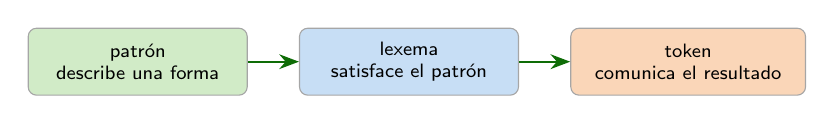
\begin{tikzpicture}[node distance=.65cm]
\node[mini, fill=pastelgreen, text width=2.5cm] (a) {patrón\\describe una forma};
\node[mini, fill=pastelblue, right=of a, text width=2.5cm] (b) {lexema\\satisface el patrón};
\node[mini, fill=pastelpeach, right=of b, text width=2.7cm] (c) {token\\comunica el resultado};
\draw[arrow] (a) -- (b);
\draw[arrow] (b) -- (c);
\end{tikzpicture}
\end{center}

\vfill
\end{frame}

\begin{frame}{¿Para qué sirve un atributo?}
\vfill

\begin{center}
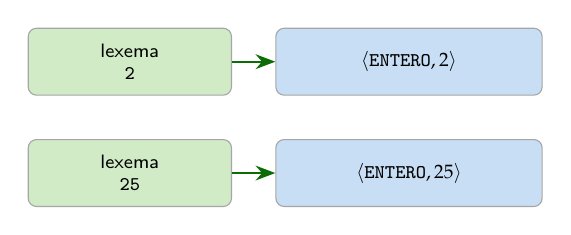
\begin{tikzpicture}[node distance=.55cm]
\node[mini, fill=pastelgreen, text width=2.3cm] (a) {lexema\\\texttt{2}};
\node[mini, fill=pastelblue, right=of a, text width=3.1cm] (b) {\(\langle\texttt{ENTERO},2\rangle\)};
\node[mini, fill=pastelgreen, below=of a, text width=2.3cm] (c) {lexema\\\texttt{25}};
\node[mini, fill=pastelblue, right=of c, text width=3.1cm] (d) {\(\langle\texttt{ENTERO},25\rangle\)};
\draw[arrow] (a) -- (b);
\draw[arrow] (c) -- (d);
\end{tikzpicture}
\end{center}

\bigskip

\begin{block}{Mismo nombre, distinta aparición}
El nombre \texttt{ENTERO} comunica la categoría; el atributo distingue el valor concreto. De manera semejante, un token \texttt{ID} puede conservar el texto del identificador o una referencia a información asociada.
\end{block}

\bigskip

\begin{center}
\small Algunos operadores y signos de puntuación no necesitan atributo: su nombre ya comunica la información requerida.
\end{center}

\vfill
\end{frame}

\begin{frame}{Trabajo con el cuadernillo}
\vfill

\begin{center}
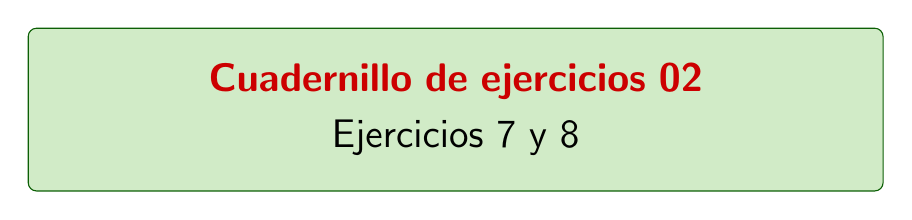
\begin{tikzpicture}
\node[
  idea,
  fill=pastelgreen,
  text width=.82\textwidth,
  inner sep=13pt,
  font=\Large
]
{\actividad{Cuadernillo de ejercicios 02}\\[2pt]
Ejercicios 7 y 8};
\end{tikzpicture}
\end{center}

\bigskip

\begin{itemize}
\item \textbf{Esencial --- Ejercicio 7:} relacionar token, lexema, patrón y atributo.
\item \textbf{Esencial --- Ejercicio 8:} analizar el fragmento ilustrativo \texttt{total = 25;}.
\end{itemize}

\vfill
\end{frame}

\begin{frame}{El analizador sintáctico solicita tokens}
\vfill

\begin{center}
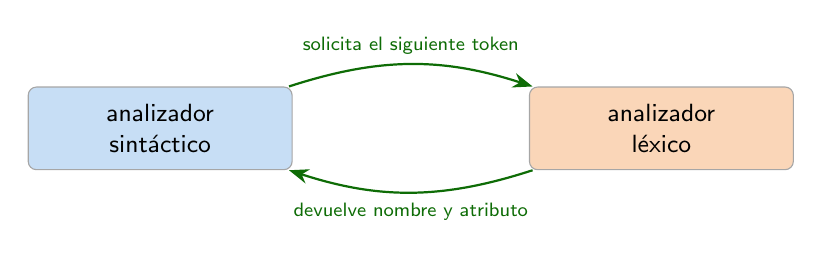
\begin{tikzpicture}[node distance=3cm]
\node[bloque, fill=pastelblue, text width=3cm] (a) {analizador\\sintáctico};
\node[bloque, fill=pastelpeach, right=of a, text width=3cm] (b) {analizador\\léxico};
\draw[arrow, bend left=18] (a) to node[above, font=\scriptsize]{solicita el siguiente token} (b);
\draw[arrow, bend left=18] (b) to node[below, font=\scriptsize]{devuelve nombre y atributo} (a);
\end{tikzpicture}
\end{center}

\bigskip

\begin{block}{Una interfaz frecuente}
El analizador léxico consume sólo los caracteres necesarios para reconocer el siguiente lexema y devolver su token.
\end{block}

\bigskip

\begin{center}
\term{La salida léxica debe tener la forma que espera el analizador sintáctico.}
\end{center}

\vfill
\end{frame}

\begin{frame}{Qué especificamos y qué apoya Lark}
\vfill

\begin{columns}[T,onlytextwidth]
\begin{column}{.48\textwidth}
\begin{block}{El equipo especifica}
\small
\begin{itemize}
\item qué categorías reconoce el lenguaje;
\item qué forma tiene cada categoría;
\item qué información debe conservar cada token.
\end{itemize}
\end{block}
\end{column}
\begin{column}{.48\textwidth}
\begin{block}{Lark apoya}
\small
\begin{itemize}
\item la lectura de la entrada;
\item el reconocimiento según las reglas dadas;
\item la producción de tokens para observar o analizar.
\end{itemize}
\end{block}
\end{column}
\end{columns}

\bigskip

\begin{center}
\texttt{parser=None}\qquad
\texttt{lexer="basic"}\qquad
\texttt{lex()}
\end{center}

\begin{center}
\small Esta configuración permite observar el analizador léxico de manera independiente.
\end{center}

\begin{center}
\small Primero la usaremos para construir el lexer de \textsc{IMP}; la práctica extenderá sus reglas para \textsc{IMP++}.
\end{center}

\vfill
\end{frame}

\begin{frame}{Confusiones que debemos evitar}
\vfill

\begin{center}
\scriptsize
\renewcommand{\arraystretch}{1.2}
\begin{tabular}{|L{.39\textwidth}|L{.47\textwidth}|}
\hline
\textbf{Confusión} & \textbf{Corrección} \tabularnewline
\hline
Lexema y patrón son lo mismo. & El lexema es concreto; el patrón describe una forma. \tabularnewline
\hline
El léxico recibe tokens y produce caracteres. & Recibe caracteres y produce tokens. \tabularnewline
\hline
Dos tokens \texttt{ID} tienen el mismo lexema. & Pueden compartir nombre y tener lexemas y atributos distintos. \tabularnewline
\hline
La optimización repara la sintaxis. & Transforma una representación válida sin cambiar su comportamiento. \tabularnewline
\hline
El \textsc{C} generado ya es ejecutable. & Debe continuar por un compilador de \textsc{C}. \tabularnewline
\hline
Lark decide las categorías del lenguaje. & Lark aplica las categorías y reglas especificadas por el equipo. \tabularnewline
\hline
\end{tabular}
\end{center}

\vfill
\end{frame}

\begin{frame}{Trabajo con el cuadernillo}
\vfill

\begin{center}
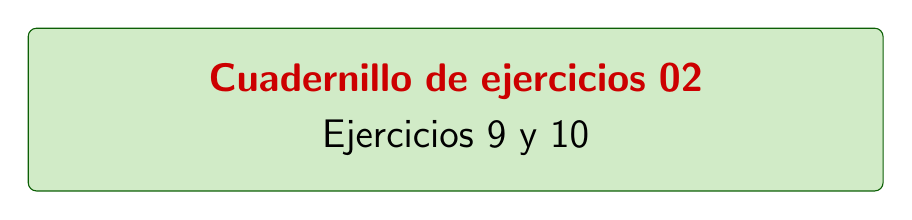
\begin{tikzpicture}
\node[
  idea,
  fill=pastelgreen,
  text width=.82\textwidth,
  inner sep=13pt,
  font=\Large
]
{\actividad{Cuadernillo de ejercicios 02}\\[2pt]
Ejercicios 9 y 10};
\end{tikzpicture}
\end{center}

\bigskip

\begin{itemize}
\item \textbf{Esencial --- Ejercicio 9:} completar la comunicación para solicitar el siguiente token.
\item \textbf{Extensión --- Ejercicio 10:} detectar y corregir confusiones del repaso completo.
\end{itemize}

\vfill
\end{frame}

\begin{frame}{Conclusión}
\vfill

\begin{center}
\resizebox{.96\textwidth}{!}{%
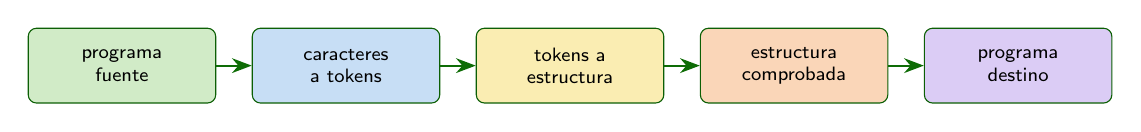
\begin{tikzpicture}[node distance=.45cm]
\node[paso, fill=pastelgreen, text width=2.1cm] (a) {programa\\fuente};
\node[paso, fill=pastelblue, right=of a, text width=2.1cm] (b) {caracteres\\a tokens};
\node[paso, fill=pastelyellow, right=of b, text width=2.1cm] (c) {tokens a\\estructura};
\node[paso, fill=pastelpeach, right=of c, text width=2.1cm] (d) {estructura\\comprobada};
\node[paso, fill=pastelviolet, right=of d, text width=2.1cm] (e) {programa\\destino};
\draw[arrow] (a) -- (b);
\draw[arrow] (b) -- (c);
\draw[arrow] (c) -- (d);
\draw[arrow] (d) -- (e);
\end{tikzpicture}%
}
\end{center}

\bigskip

\begin{block}{Idea de cierre}
El compilador organiza transformaciones mediante fases con responsabilidades e interfaces claras. El análisis léxico inicia el recorrido interno: reconoce lexemas, produce tokens y comunica la información que necesita la fase sintáctica.
\end{block}

\bigskip

\begin{center}
\term{Cada contrato se implementará primero para \textsc{IMP} y se extenderá después para \textsc{IMP++}.}
\end{center}

\vfill
\end{frame}

\begin{frame}{Referencias}
\vfill

\tiny
\begin{enumerate}
\item Soto Romero, M. y Reyes Cabello, A. L. (2026). \textit{Programación de Sistemas. Nota de clase 02: Estructura y fases de un compilador}. Colegio de Ciencia y Tecnología, UACM.
\item Soto Romero, M. y Reyes Cabello, A. L. (2026). \textit{Programación de Sistemas. Nota de clase 03: Fundamentos del análisis léxico}. Colegio de Ciencia y Tecnología, UACM.
\item Soto Romero, M. y Reyes Cabello, A. L. (2026). \textit{Programación de Sistemas. Cuadernillo de ejercicios 02: Del software de sistemas al análisis léxico}. Colegio de Ciencia y Tecnología, UACM.
\item Aho, A. V., Lam, M. S., Sethi, R., y Ullman, J. D. (2008). \textit{Compiladores: principios, técnicas y herramientas} (2.\textsuperscript{a} ed.). Pearson Educación. ISBN 978-970-26-1133-2.
\item Thain, D. (2026). \textit{Introduction to Compilers and Language Design} (2.\textsuperscript{a} ed.). University of Notre Dame.
\item Vilar Torres, J. M. (2010). \textit{Estructura de los compiladores e intérpretes}. Universitat Jaume I.
\item Vilar Torres, J. M. (2010). \textit{Analizador léxico}. Universitat Jaume I.
\end{enumerate}

\vfill
\end{frame}

\end{document}
